% Compile twice with: pdflatex Review_Report_Class_Example.tex
% Keep ssnreview.cls and the optional logo in the same folder.
\documentclass{ssnreview}

\projecttitle{TITLE OF THE PROJECT}
\reviewnumber{REVIEW REPORT -- I}
\students{%
  Student Name 1 (Register No.)\\
  Student Name 2 (Register No.)\\
  Student Name 3 (Register No.)\\
  Student Name 4 (Register No.)}
\supervisor{Dr./Mr./Ms. Supervisor Name}
\department{Department of Computer Science and Engineering}
\institution{Sri Sivasubramaniya Nadar College of Engineering}
\academicyear{2026--2027}
\collegelogo{ssn-logo.png}

\begin{document}
\makereviewtitle
\reviewfrontmatter

\begin{reviewabstract}
Write a concise summary in approximately 200--300 words. Include the background,
problem, proposed approach, results, and main contribution.

\keywords{Keyword 1; Keyword 2; Keyword 3; Keyword 4}
\end{reviewabstract}

\chapter{Introduction}
Introduce the project domain, motivation, context, and significance.
\section{Background} Describe the required technical background.
\section{Motivation} Explain why this work is important.
\section{Objectives}
\begin{enumerate}[label=\arabic*.]
  \item To design and develop \ldots
  \item To implement and evaluate \ldots
  \item To compare the proposed solution with \ldots
\end{enumerate}
\section{Scope} State the project boundaries.


\chapter{Related Work}
Critically compare relevant work and cite sources, for example \cite{samplepaper}.
\begin{table}[H]
\centering\caption{Summary of related work}\label{tab:related-work}\small
\begin{tabularx}{\textwidth}{>{\centering\arraybackslash}p{0.7cm} p{2.8cm} X X X}
\toprule
\textbf{S.No.} & \textbf{Author/Year} & \textbf{Proposed Method} & \textbf{Key Findings} & \textbf{Limitations}\\
\midrule
1 & Author et al. (2025) & Describe the method. & State the result. & State the gap.\\
2 & Author et al. (2024) & Describe the method. & State the result. & State the gap.\\
\bottomrule
\end{tabularx}
\end{table}
\textcolor{red}{
  Summary of Related Works table is mandatory and it should list the mainly 
  refered documents for your work. 
  Don't change the table column headings.
}

\section{Research Gap} Identify the gap addressed by this project.

\chapter{Problem statement}
Present a precise, measurable problem with inputs, outputs, constraints, and criteria.

\chapter{Justification for the problem formulation}
Justify the technical need, relevance, feasibility, and expected impact.
\section{Need for the Proposed Work} Explain why the problem deserves attention.
\section{Feasibility} Discuss technical, operational, economic, and schedule feasibility.
\section{Expected Contribution} State the anticipated novelty or improvement.

\chapter{Methodology}
Describe the complete workflow used to achieve the objectives.
%\section{Proposed Workflow}
%\begin{enumerate}[label=\textbf{Step \arabic*:}]
%  \item Collect or prepare data and resources.
%  \item Preprocess inputs and extract relevant features.
%  \item Design and implement the proposed system.
%  \item Train, test, validate, or deploy the solution.
%  \item Evaluate it using suitable metrics and baselines.
%\end{enumerate}

%\section{Tools and Technologies}
%\begin{table}[H]
%\centering\caption{Proposed tools and technologies}
%\begin{tabularx}{0.9\textwidth}{p{4cm} X}
%\toprule \textbf{Category} & \textbf{Tool/Technology}\\ \midrule
%Programming language & Python / Java / Other\\
%Frameworks and libraries & Add relevant frameworks and libraries\\
%Database or storage & Add the proposed platform\\
%Development platform & Add IDE, cloud, container, or hardware details\\
%\bottomrule
%\end{tabularx}
%\end{table}
%\section{Evaluation Plan} Specify datasets, experiments, baselines, and metrics.

\section{Architectural Design for Proposed System}
Explain components, responsibilities, interfaces, data flow, and deployment.
\begin{figure}[H]
\centering
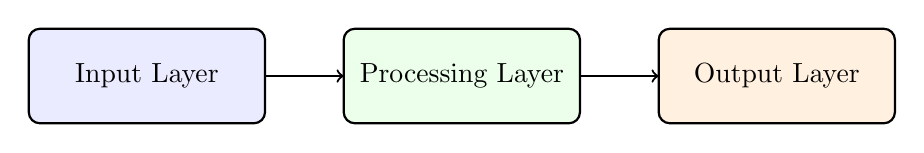
\begin{tikzpicture}
  \draw[rounded corners,thick,fill=blue!8] (0,0) rectangle (3,1.2);
  \node at (1.5,0.6) {Input Layer};
  \draw[->,thick] (3,0.6) -- (4,0.6);
  \draw[rounded corners,thick,fill=green!8] (4,0) rectangle (7,1.2);
  \node at (5.5,0.6) {Processing Layer};
  \draw[->,thick] (7,0.6) -- (8,0.6);
  \draw[rounded corners,thick,fill=orange!12] (8,0) rectangle (11,1.2);
  \node at (9.5,0.6) {Output Layer};
\end{tikzpicture}
\caption{High-level architecture of the proposed system}\label{fig:architecture}
\end{figure}

\section{Modules}
For each module, specify its purpose, inputs, processing, outputs, and dependencies.
\subsection{Module 1: Data/Input Management} Describe input handling and preprocessing.
\subsection{Module 2: Core Processing} Describe the main algorithm or business logic.
\subsection{Module 3: User Interface and Output} Describe interaction and reporting.
\subsection{Module 4: Testing and Evaluation} Describe testing and validation.

\chapter{Project timeline chart}
\begin{figure}[H]
\centering
\resizebox{\textwidth}{!}{%
\begin{ganttchart}[hgrid,vgrid,time slot format=isodate-yearmonth,time slot unit=month,
 title label font=\bfseries\footnotesize,bar label font=\small,
 bar/.append style={fill=blue!45},milestone/.append style={fill=red}]
 {2026-08}{2027-03}
\gantttitlecalendar{year, month=shortname}\\
\ganttbar{Literature survey}{2026-08}{2026-09}\\
\ganttbar{Problem formulation}{2026-09}{2026-10}\\
\ganttbar{System design}{2026-10}{2026-11}\\
\ganttbar{Implementation}{2026-11}{2027-01}\\
\ganttbar{Testing and evaluation}{2027-01}{2027-02}\\
\ganttbar{Documentation}{2027-02}{2027-03}\\
\ganttmilestone{Final submission}{2027-03}
\end{ganttchart}}
\caption{Project timeline}\label{fig:timeline}
\end{figure}


%\chapter{Reference}
\begin{thebibliography}{99}
\bibitem{samplepaper} A. Author and B. Author, "Title of the research paper", \textit{Journal or Conference Name}, vol.~1, no.~1, pp.~1--10, 2025.
DOI: \url{https://doi.org/10.3844/jcssp.2021.610.623}.
\bibitem{r1} Wu, F., Souza, A., Zhang, T., Fifty, C., Yu, T., and Weinberger, K, "Simplifying graph convolutional networks", \textit{In the International Conference on Machine Learning"}, pages 6861–6871. Available from \url{https://proceedings.mlr.press/v97/wu19e.html}
\bibitem{r2} Zhang, Z. and Fink, O, "Algorithm-informed graph neural networks for leakage detection and localization in water distribution networks", \textit{Reliability Engineering \& System Safety}, page 111494. DOI: \url{https://doi.org/10.1016/j.ress.2025.111494}
\bibitem{r3}, Zhao, F., Liu, J., Zhang, S., Tao, L., Wang, J., Zhang, Z., and Li, N, "A novel method for detecting the leakage duration of water pipe network based on the anchor box mechanism", \textit{In 2025 IEEE 2nd International Conference on Energy and Electrical Engineering (EEE)}, pages 1–5. IEEE, DOI: \url{https://doi.org/10.1109/eee64897.2025.11162744}
\bibitem{samplebook} C. Author, \textit{Title of the Book}, 2nd ed. City, Country: Publisher, 2024.
\bibitem{samplewebsite} Organization Name, ``Title of the webpage,'' 2026. [Online]. Available: \url{https://example.com}. [Accessed: 7-Aug-2026].
\end{thebibliography}

\end{document}